V celé sekci je zvolena přesnost na 3 desetinná místa. Přesnější hodnoty jsou k nahlédnutí v přiloženém skriptu. Pro zachování přehlednosti nejsou v práci všechny výstupy z Maplu.\\
Zadána byla spodní a horní hranice nepropustného pásma $f_{-s},fs$\,[Hz], spodní a horní hranice propustného pásma $f_{-p},f_p$\,[Hz], maximální útlum v propustném pásmu $a_p$\,[dB] a minimální útlum v~nepropustném pásmu $a_s$\,[dB]. Toleranční schéma definuje oblasti, do kterých nesmí charakteristika filtru zasáhnout. Pro návrh pásmové propusti 4. řádu s Cauerovou aproximací typu C byly zvoleny parametry tolerančního schématu $f_{-s} = 60$\,kHz, $f_{-p} = 150$\,kHz, $f_p = 190$\,kHz, $f_s = 280$\,kHz, $a_p = 1$\,dB a $a_s = 80$\,dB. Všechny parametry musí být kladná reálná čísla a $f_{-s}$ <  $f_{-p}$ < $f_p$ < $f_s$ a $a_p$ < $a_s$. 
\begin{align}
f_{-s} &= \frac{\sqrt{\Delta{fs}^2+4f\_m ^2}-\Delta{fs}}{2}\\
f_{-p} &= \frac{\sqrt{\Delta{fp}^2+4f\_m ^2}-\Delta{fp}}{2}\\
f_p &= \frac{\sqrt{\Delta{fp}^2+4f\_m ^2}+\Delta{fp}}{2}\\
f_s &= \frac{\sqrt{\Delta{fs}^2+4f\_m ^2}+\Delta{fs}}{2}
\end{align}
Funkcí $BP2NLP$ byla provedena transformace tolerančního schematu nesymetrické pásmové propusti (PP) na toleranční schema normované dolní propusti (NDP). Byl spočítán nový kmitočet pro horní hranici nepropustného pásma $f_s = 101.786$\,kHz, geometrický střed propustného pásma $f_m = 168.819$\,kHz, šířka propustného pásma $\Delta{f_p} = 40$\,kHz a šířka nepropustného pásma $\Delta{f_s} = 178.314$\,kHz. Byl obdržen kmitočet hranice nepropustného pásma normované dolní propusti (NDP) $Os = 4.455$\,1/s.
\begin{figure}[h]
\centering
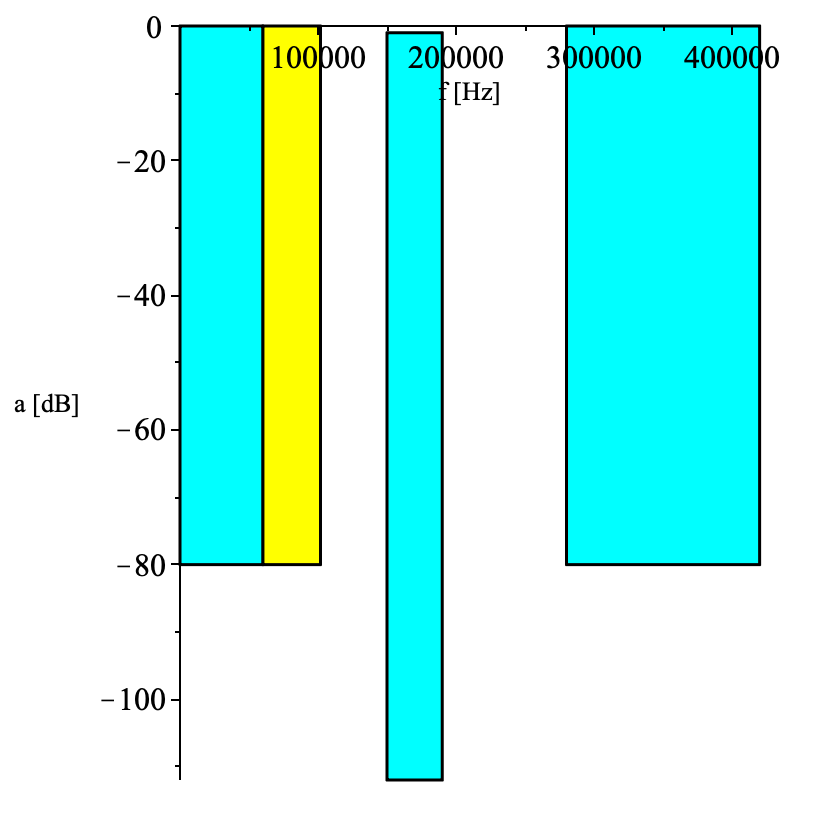
\includegraphics[scale=0.45]{tolsch2.png}
\caption{Toleranční schéma navrhované pásmové propusti}
\end{figure}
\noindent Stupeň Cauerovy aproximace normované dolní propusti byl určen jako $order = 4$. Pro Cauerovu aproximaci jsou definovány tři typy --- A, B, C. Tyto typy se od sebe liší průběhem aproximační funkce. Byla zvolena aproximace typu C se shodnými zakončovacími odpory.
\noindent Dále byla funkcí $Cauer\_asnew$ určena nová hodnota útlumu v~nepropustném pásmu NDP $a_{snew} = 81.719$\,dB.
\begin{align}
asnew&= 10 \cdot log_{10}\left(1 + \left( \frac{\epsilon}{kl\_new}\right)^2\right)\\
\epsilon &= \sqrt{10^{0.1ap} - 1}\\
k &= \frac{1}{Os}\\
kl\_new &= k^{order}\left(\prod_{i=1}^{n}JacobiCD\left(\frac{(2i - 1 + m)EllipticK(k)}{order},k\right)\right)^4,
\end{align}
\noindent kde $m$ je celočíselný zbytek po dělení řádu 2 a $n$ celočíselný výsledek dělení. Jakobiho eliptických funkcí je 12 a vycházejí ze škálování na jednotkové elipse (cos $\phi$, sin $\phi$ se~neváží k jednotkovému kruhu, ale k elipse). \\
\\
Následně byl spočten koeficient nejvyšší mocniny polynomu ve jmenovateli přenosové funkce $Gc = 94.811$, póly $P$ a nuly $Z$ přenosové funkce pomocí funkce $CauerCPolesZeros$. Počet pólů je dán řádem filtru $order$ a počet nul pro aproximaci typu C je roven $order = 2$. Dále byla spočtena Caurerova aproximace typu C~---~provozní činitel přenosu $G$ jako racionální lomená funkce $G(p) = 1/H(p)$, charakteristická funkce $chf$ jako $\Phi(p)$ s nulami a póly na imaginární ose. Charakteristická funkce má shodný jmenovatel s $G(p)$.
\begin{equation}
P = 
\begin{bmatrix}
0.478 + 0.343 I & -0.478 - 0.343 I & -0.161 + 0.983 I & -0.161 - 0.983 I
\end{bmatrix}
\end{equation}
\begin{align}
Z &=
\begin{bmatrix}
5.706 I & -5.706 I
\end{bmatrix}\\
G &= \frac{94.881p^4+121.138p^3+156.142p^2+100.507p+32.556}{p^2+32.556}\\
chf &= \frac{(94.811p^2+78.754)p^2}{p^2+32.556}
\end{align}
\begin{figure}[h]
\centering
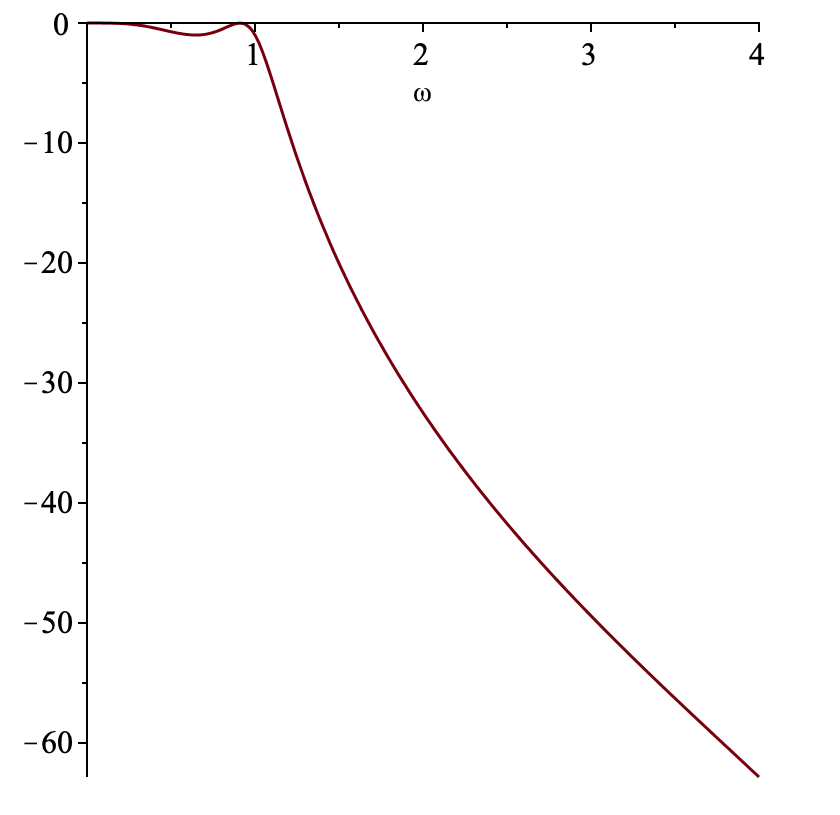
\includegraphics[scale=0.45]{sch02.png}
\caption{Modulová frekvenční charakteristika NDP}
\end{figure}
\noindent Charakteristika byla vykreslena z přenosu funkcí $MagnitudeHdB$, která vypočte modul přenosu podle předpisu |H(j$\omega)$| a výsledek převede na $20 \cdot log_{10} |H(p)|$.
\subsection{Příčkové LC filtry}\label{s:LC}
Pasivní dolní propust je realizována zapojením induktoru ke vstupnímu napětí a k~této větvi je následně zapojen paralelně rezistor. Pasivní horní propust má ke vstupu připojený sériově rezistor a poté k~této větvi paralelně induktor. \\
\\
K realizaci filtrů vyšších řádů se užívají $\pi$ nebo T~články s LC prvky. Podle Vedrala a Svatoše \cite{8} musí být při návrhu filtru zohledněn vnitřní odpor zdroje $R_s$ a zatěžovací odpor $R_L$. LC filtry jsou tedy dvojitě zakončeny. Indukčnosti a kapacity prvků se určí z rovnic pro normované kapacity a indukčnosti. Normované hodnoty budou vypočteny pro mezní kmitočet $\omega _0 = 1/\sqrt{LC}$ a pro zatěžovací odpor $R_L$. Hodnoty prvků lze pro požadovanou aproximaci odečíst z tabulek. Pro LC filtry se používá kmitočtová oblast $10^{3}$\,Hz--$10^{2}$\,MHz.\\
\\
\begin{figure}[h]
\centering
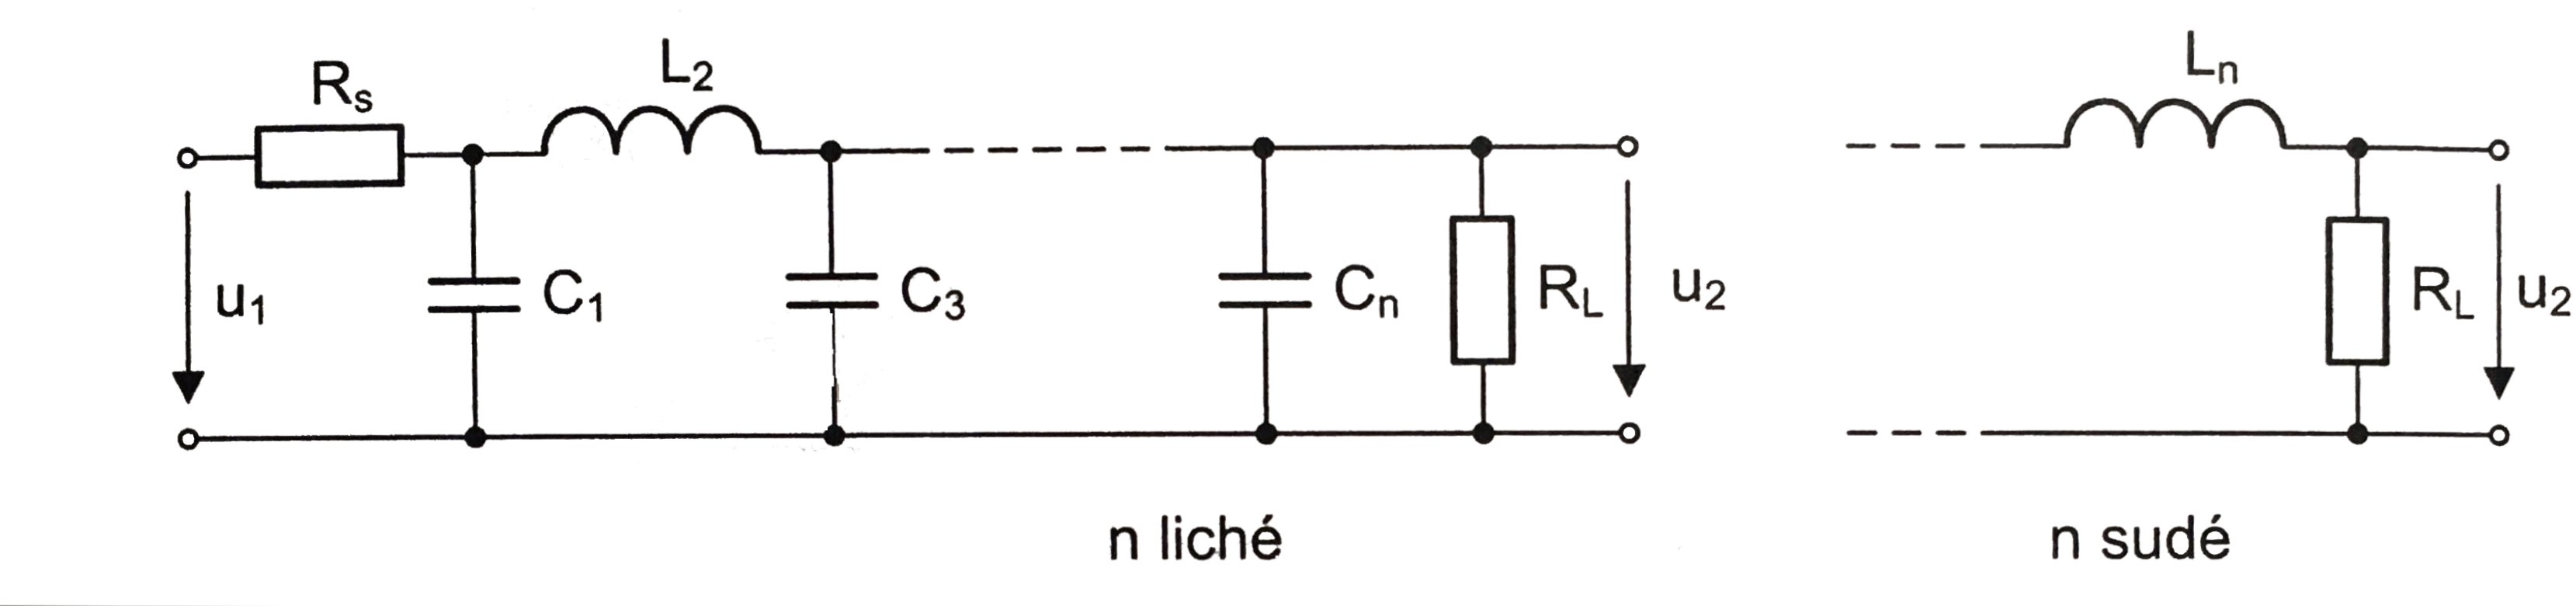
\includegraphics[scale=0.125]{piclanky.png}
\caption[Pasivní dolní propust n-tého řády s $\pi$ články]{Pasivní dolní propust n-tého řády s $\pi$ články \cite{8}}
\end{figure}
\begin{figure}[h]
\centering
\includegraphics[scale=0.078]{tclanky.png}
\caption[Pasivní dolní propust n-tého řády s T články]{Pasivní dolní propust n-tého řády s T články \cite{8}}
\end{figure}
\subsection{Gyrátory}\label{s:GYR}
\noindent K převodu induktoru na zapojení s kapacitorem byla použita struktura označovaná jako gyrátor. Jde o náhradu původního obvodu s induktorem vhodným uspořádáním rezistorů a kapacitorů tak, že výsledná impedance vypadá jako induktor. Jelikož po této substituci v obvodu zůstanou jen R,C prvky, jedná se o ARC syntézu. \\
\\
 Gyrátor je podle Martinka, Boreše a Hospodky \cite{12} typ invertoru. Pro invertory platí, že jejich vstupní impedanci lze napsat ve tvaru\begin{equation}
Z_{vst} = \frac{a_{12}}{a_{21}}\frac{1}{Z_L} = \frac{a_{12}}{a_{21}}Y_L.
\end{equation}
Pokud jsou parametry $a_{12}, a_{21}$ reálné a kladné, hovoříme o gyrátoru. Symbol gyrátoru je na obrázku \ref{s:G}. Gyrátor se nejúspěšněji dá realizovat paralelním spojením dvou napětím řízených zdrojů proudu s opačným znaménkem. Zapojení s OTA odpovídá dvěma zesilovačům, jeden s uzemněnou zápornou a druhý s uzemněnou kladnou svorkou vstupu. Výstup prvního ze zesilovačů je propojen s volnou vstupní svorkou druhého a naopak.
\begin{figure}[h]
\centering
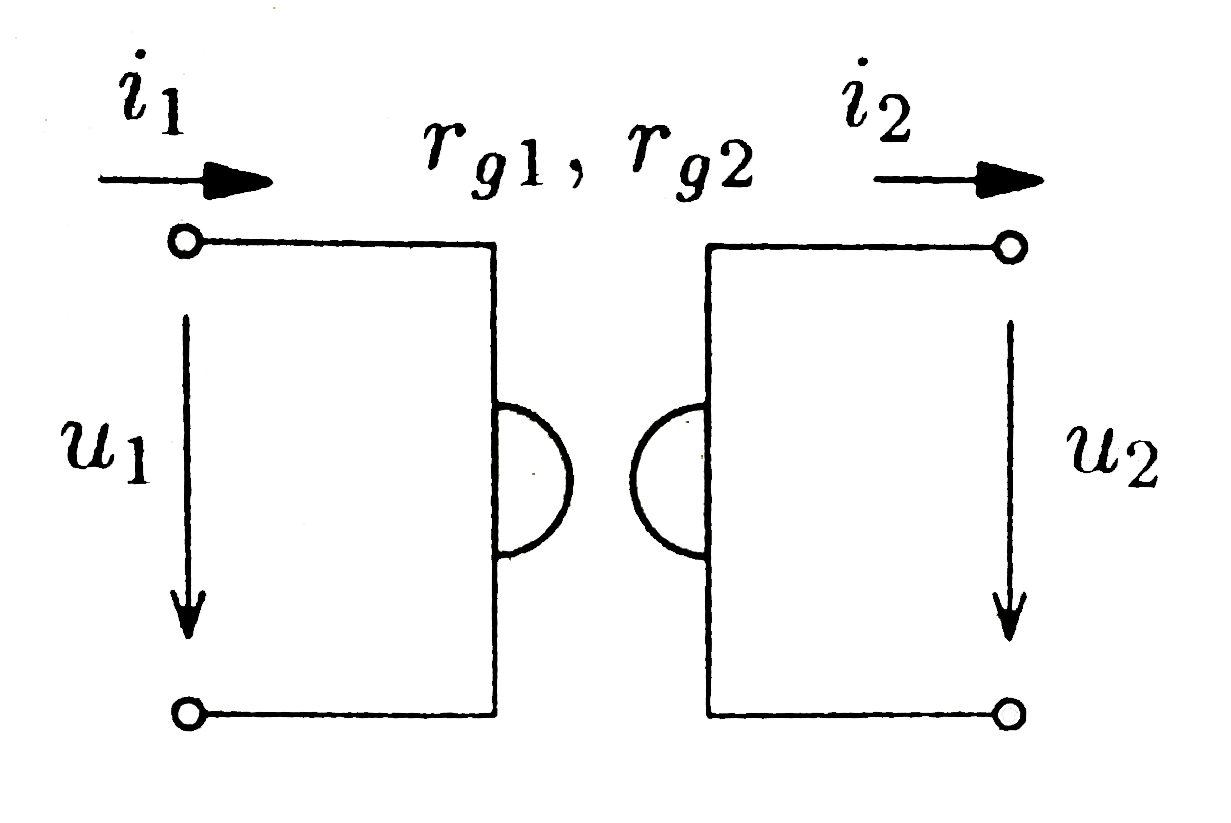
\includegraphics[scale=0.095]{gyr.png}
\caption{Definice gyrátoru \label{s:G}}
\end{figure}
Podle Schaumanna a Valkenburga \cite{13} nelze gyrátor dobře realizovat s obyčejnými operačními zesilovači, běžně se používají \textit{General Impedance Converters} (GIC). Převod induktoru na jiné zapojení s ekvivalentní impedancí má praktické využití v integrovaných obvodech, kde jsou kapacitory preferovány nad induktory kvůli malým rozměrům. Navíc se induktory musí složitě vyrábět na danou hodnotu. V návrhu integrovaných obvodů se také většinou nepoužívají rezistory kvůli místu na čipu, které zabírají. \\
\\
Gyrátor je principielně spojení invertujícího a neinvertujícího napětím řízeného zdroje proudu, a proto ho lze realizovat snadno s transkonduktančními zesilovači. Na obrázku \ref{s:GO} jsou podle Schaumanna a Valkenburga \cite{13} znázorněny dva gyrátory s kapacitorem. 
\begin{figure}[h]
\centering
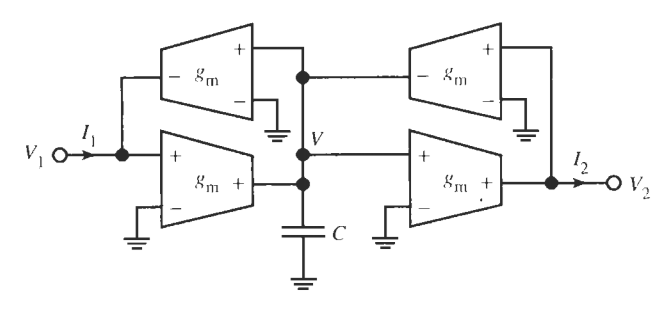
\includegraphics[scale=0.4]{gyrator.png}
\caption[Neuzemněný induktor realizovaný kapacitorem a dvěma gyrátory]{Neuzemněný induktor realizovaný kapacitorem a dvěma gyrátory \label{s:GO}}
\end{figure}
Obvodovou analýzou v uzlu V byla obdržena rovnice
\begin{align}
pCV &= g_mV_1 - g_mV_2
\end{align}
a dva proudy na výstupu
\begin{align}
I_1 = I_2 = g_mV.
\end{align}
Zkombinování rovnic a eliminace V vede k rovnici neuzemněného induktoru mezi napětími $V_1$ a $V_2$.
\begin{align}
I_1 = I_2 = \frac{g_m^2}{pC}(V_1 - V_2) = \frac{1}{pL}(V_1 - V_2)
\end{align}
Z rovnice lze snadno odvodit, že kapacita kondenzátoru použitého jako náhrada zapojení induktoru v zapojení s OTA je rovna $C_L = L g_m ^2$. \\
\subsection{Výpočet prvků LC filtru a přenosových funkcí}\label{s:VYP}
\noindent Funkcí $DroppNLP$ byly vypočteny prvky LC příčkového filtru typu normovaná dolní propust (NDP). Zakončení bylo zvoleno standardní (\textit{common}), odpory o hodnotě 1\,$\Omega$, směr zpracování od posledního prvku (\textit{rear}), s T strukturou (začíná zepředu podélným induktorem). Standardní (\textit{common}) zakončení je oboustranné ($R_1~\neq~0, R_z~\neq~\infty$). Výstupem funkce je LC struktura s orientací prvků ve větvi podélně (\textit{direct}) nebo příčně (\textit{shunt}).
\MapleOutput{block (1), [orientation = direct, elements = {L1 = 1.571}, Z = p L1]}
\MapleOutput{block (2), [orientation = shunt, elements = {C1 = 1.542}, Z = \frac{1}{pC1}]}
\MapleOutput{block (3), [orientation = direct, elements = {C1 = 0.02, L1 = 1.522}, Z = \frac{1}{\frac{1}{pL1} + pC1}]}
\MapleOutput{block (4), [orientation = shunt, elements = {C1 = 1.545}, Z = \frac{1}{pC1}]}
\noindent Přenosová funkce pasivních a aktivních struktur filtru byla spočtena funkcí $MakeH$. Byl spočten  napěťový i~výkonový přenos.
\begin{align}
H_{NLPV} &= \frac{p^2  + 32.556}{190.352p^4  + 242.742p^3  + 312.889p^2  + 201.21p + 65.112}\\
H_{NLP} &= \frac{p^2  + 32.556}{95.176p^4 + 121.371p^3 + 156.444p^2 + 100.605p + 32.556}
\end{align}
\noindent Z rozložení pólů je patrné, že obě přenosové funkce jsou stabilní.
\begin{align}
190.352s_1^4 + 242.742s_1^3 + 312.889s_1^2 + 201.21s_1 + 65.112 &= 0 \\
95.176s_2^4 + 121.371s_2^3 + 156.444s_2^2 + 100.605s_2 + 32.556 &= 0
\end{align}
\begin{align}
s_1 &= {-0.477 - 0.3431 I}, {-0.477 + 0.343 I}, {-0.161 - 0.983 I}, {-0.161 + 0.983 I}\\
s_2 &= {-0.477 - 0.3431 I}, {-0.477 + 0.343 I}, {-0.161 - 0.983 I}, {-0.161+ 0.983 I}
\end{align}
\begin{figure}[h]
\centering
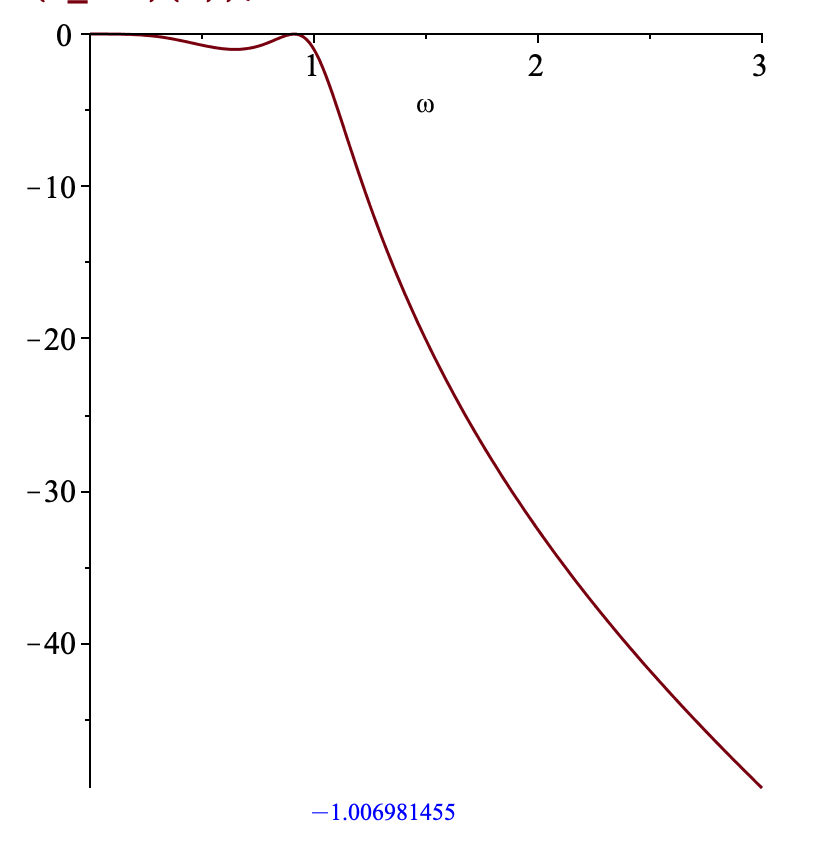
\includegraphics[scale=0.45]{sch022.png}
\caption{Modulová frekvenční charakteristika NDP - LC příčkový filtr}
\end{figure}
\noindent Hodnota přenosové funkce v 1 byla vyhodnocena jako $-1.007$.\\
\noindent Byla provedena transformace hodnot prvků normované dolní propusti (NDP) na~pásmovou propust (PP). Zakončovací rezistor byl zvolen 1\,$\Omega$, další dva parametry funkce značí spodní a horní hranici propustného pásma.\\
Prvky v první větvi obvodu byly vyčísleny jako $C_1 = 1.422$e-7\,F, $L1 = 6.252$e-6\,H, v druhé větvi $C_2 = 6.135$e-6\,F, $L_2 = 1.449$e-7\,H. Pro třetí větev $C_3 = 8.031$e-8\,F, $C_4 = 1.468$e-7\,F, $L_3 = 1.107$e-5\,H, $L_4 = 6.055$e-6\,H a pro čtvrtou $C_5 = 6.149$e-6\,F, $L_5 = 1.445$e-7\,H.\\
\noindent Vygenerovaná struktura je popsána na obrázku \ref{s:SCHEM}.\\
\\
\begin{figure}[h]
\centering
\resizebox{12cm}{!}{
\figppp{Circuit(1)}{5.566}{2.075}{}{}}
\caption{Schéma LC příčkové struktury \label{s:SCHEM}}
\end{figure}
\noindent Byly nastaveny jakosti cívek v LC příčkové struktuře na konečnou hodnotu. Funkce $MakeRealL$ zařadí do výsledné LC příčkové struktury sériově rezistory k induktorům podle zadaného činitele jakosti $Q$ a zadaného kmitočtu (ten odpovídá u pásmové propusti geometrickému středu propustného pásma --- nebo je možno zadat obě hranice propustného pásma). Byl zvolen činitel jakosti 100. Činitel jakosti je dán převrácenou hodnotou poměrné šířky pásma
\begin{equation}
Q = \frac{1}{B} = \frac{\omega_s}{\delta \omega},
\end{equation}
kde B je poměrná šířka pásma, $\delta \omega = \omega_2 - \omega_1$ a $\omega_s = \sqrt{\omega_1\omega_2}$. $\omega_1$ a $\omega_2$ zde jsou mezní kruhové kmitočty odpovídající poklesu přenosu filtru o 3\,dB.\\
\\
Pro kmitočtové pásmo stovky kHz až jednotky MHz v závislosti na typu jádra a kvalitě materiálu lze dosahovat hodnoty činitele jakosti cca 1000 a hodnoty indukčnosti řádově 100\,$\upmu$H až 10\,mH. Pro činitel jakosti se zde uplatňuje kmitočtová závislost $Q = \omega L/R$. Pro kmitočtové pásmo do 10\,kHz hodnoty činitele jakosti klesají řádově na hodnoty 10 pro velké hodnoty L. Výpočet sériového odporu je proveden podle předpisu $R_s~=~L1~\cdot~2~\pi~f/Q$. Pro první větev je $R_{s1} = 0.066$\,$\Omega$, pro druhou $R_{s2} = 0.002$\,$\Omega$, pro třetí $R_{s3} = 0.117$\,$\Omega$ a $R_{s4} = 0.064$\,$\Omega$.\\
\\
\noindent Byl spočten přenos pro LC strukturu bez a s přidanými sériovými rezistory. Pro oba přenosy byla vykreslena modulová frekvenční charakteristika. Přenosové funkce zde pro svou složitost a zachování přehlednosti textu nejsou uváděny, ale jsou k nalezení v přiloženém Maple skriptu.
\begin{figure}[h]
\centering
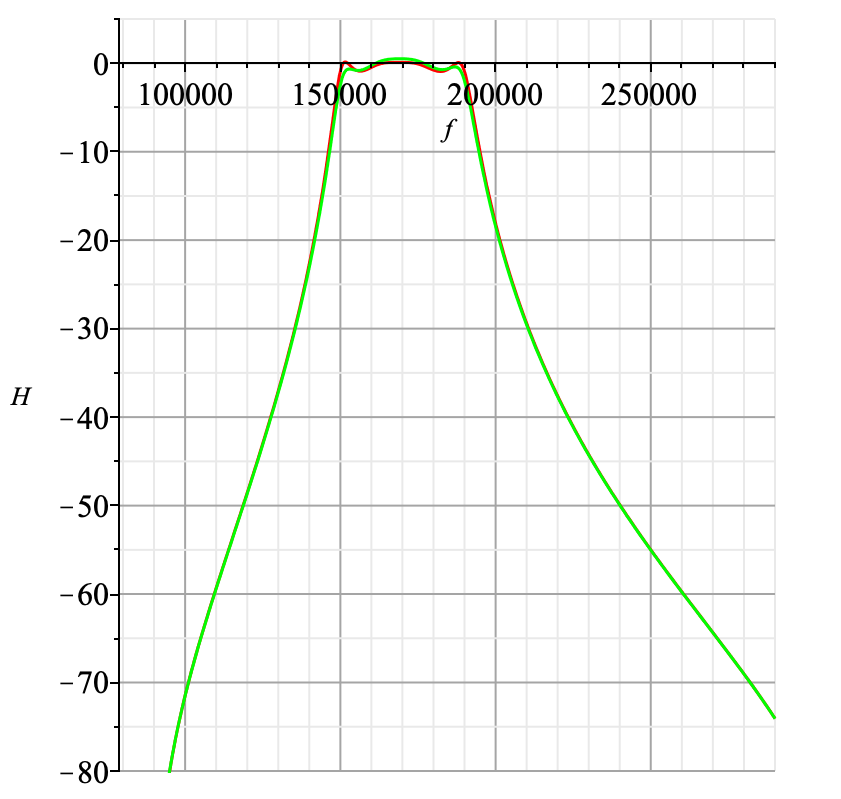
\includegraphics[scale=0.55]{modul12.png}
\caption{Modulová frekvenční charakteristika LC struktury (červená) a LC struktury s konečnou hodnotou jakostí cívek (zelená)}
\end{figure}
\begin{figure}[h]
\centering
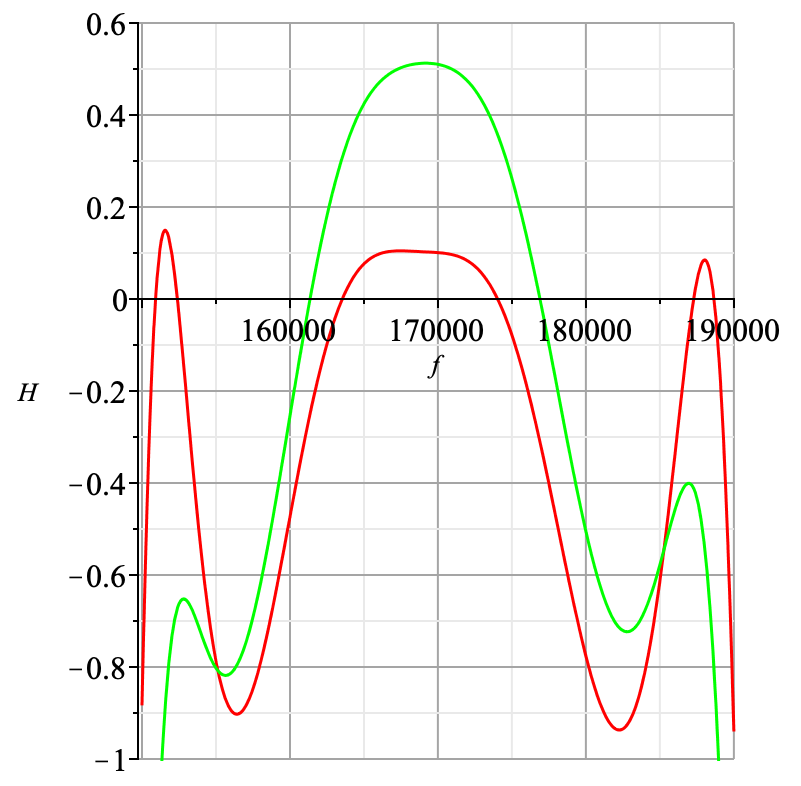
\includegraphics[scale=0.55]{modul123.png}
\caption{Přiblížená modulová frekvenční charakteristika LC struktury (červená) a LC struktury s konečnou hodnotou jakostí cívek (zelená)}
\end{figure}
\noindent Vyčíslením v $f_m \cdot 2 \pi$ Hz, kde $f_m$ je geometrický střed propustného pásma, bylo obdrženo zesílení 0.283\,dB.\\
\\
\subsection{Simulace prvků LC prototypu}\label{s:ARC}
V této sekci byl náhradou induktorů v LC prototypu za gyrátory obdržen návrh ARC filtru.\\
Zatím neodnormované prvky byly vyčísleny jako $C_1 = 1.422$e-7\,F, $C_2 = 6.135$e-6\,F, $C_3 = 1.468$e-7\,F, $C_4 = 8.031$e-8\,F, $C_5 = 6.149$e-6\,F, $L_1 = 6.252$e-6\,H, $L_2 = 1.449$e-7\,H, $L_3 = 6.055$e-6\,H, $L_4 = 1.107$e-5\,H, $L_5 = 1.445$e-7\,H, $R_1 = 1$\,$\Omega$, $R_z = 1$\,$\Omega$.\\
\\
\noindent Odnormované hodnoty kapacit získané vydělením kmitočtem $fp \cdot 2 \pi$, kde $fp$ je horní hranice propustného pásma, byly spočteny jako $C_1 = 1.191$e-13\,F, $C_2 = 5.139$e-12\,F, $C_3 = 1.23$e-13\,F, $C_4 = 6.727$e-14\,F, $C_5 = 5.151$e-12\,F.\\
\noindent Frekvenčně a impedančně odnormované odpory byly vypočteny podělením kmitočtem $fp \cdot 2 \pi$ a přibližnou hodnotou kapacity pro mikroelektronickou realizaci $C = 2$\,pF. Výsledné hodnoty jsou $R_1 = R_z = 418.828$\,$k\Omega$.\\
\noindent Využitím poznatků ze sekce \ref{s:GYR} byly dosazením do vztahu $C = L \cdot g_m^2$ s uvažováním minimální transkonduktance z datasheetu LM13700 ($g_m$ = 9600\,$\upmu$S) získány kapacity $C_{L1} = 5.762$e-10\,F, $C_{L2} = 1.335$e-11\,F, $C_{L3} = 5.58$e-10\,F, $C_{L4} = 1.02$e-15\,F, $C_{L5} = 1.332$e-11\,F.\\
\\
\noindent Výsledné hodnoty všech součástek s přesností na dvě desetinná místa jsou\\ $C1 = 11.91$\,pF, $C2 = 5.14$\,pF, $C3 = 12.3$\,pF, $C4 = 672.74$\,pF, $C5 = 5.15$\,pF, $C_{L1} = 57.62$\,nF, $C_{L2} = 133.52$\,nF, $C_{L3} = 55.8$\,nF, $C_{L4} = 1019.9$\,pF, $C_{L5} = 133.21$\,nF, $R1 = Rz = 418.83$\,$k\Omega$.
\subsection{Funkční simulace LC prototypu}\label{s:KASK}
\noindent Základní myšlenka funkční simulace LC prototypu vychází z popisu příčkové struktury grafem signálových toků a simulací tohoto grafu vhodným elektronickým obvodem. Z~aproximace bylo kaskádní syntézou získáno rozložení výsledné přenosové funkce filtru na funkce jednotlivých kaskádně řazených bloků. Kaskádně spojené dvojbrany se~vzájemně neovlivňují --- v napěťovém módu mají charakter napětím řízených zdrojů napětí a v~proudovém módu proudem řízených zdrojů proudu. Přenos celé kaskády je dán součinem přenosů jednotlivých bloků. Na jeho základě se realizuje návrh filtru jako návrh jednotlivých bloků. Návrh je proveden s bloky s~jedním OTA a po realizaci lze jednotlivé bloky modifikovat jak z hlediska struktury, tak z hlediska hodnot jednotlivých prvků vybrané struktury. Například změnou transkonduktance jednotlivých bloků pak lze variabilně modifikovat mezní kmitočet.\\
\\
\noindent Analýzou LC struktury z Maplu byly obdrženy obvodové rovnice, kde R je volitelný (fiktivní) rezistor
\begin{align}
I_1 &= \frac{1}{R_1 + pL_1 + \frac{1}{pC_1}}(U_G - U_2)\\
v_1 & = \frac{R}{R_1 + pL_1 + \frac{1}{pC_1}}(U_G - U_2)\\
U_2 &= \frac{1}{\frac{1}{pL_2} + pC_2}(I_1 - I_{3} - I_{L4} - pC_4 v_{L4})\\
U_2 &= \frac{1}{\frac{R}{pL_2} + RpC_2}(v_1 - v_{L3} - v_{L4} - RpC_4 U_{L4})\\
I_{3} &= \frac{1}{pL_3 + \frac{1}{pC_3}}(U_2 - U_3)\\
v_{L3} &= \frac{R}{pL_3 + \frac{1}{pC_3}}(U_2 - U_3)\\
v_{L4} &= \frac{1}{\frac{1}{pL_4}+pC_4}(I_1 - I_{L2} - pC_2U_2 - I_{3} - pC_4 (U_2 - U_3))\\
v_{L4} &= \frac{1}{\frac{R}{pL_4}+RpC_4}(v_1 - v_{L2} - RpC_2U_2 - v_{L3} - RpC_4 (U_2 - U_3))\\
U_3 &= \frac{1}{\frac{1}{R_z}+pC_5 + \frac{1}{pL_5}}(I_1 - I_{L2} - pC_2U_2)\\
U_3 &= \frac{1}{\frac{R}{R_z}+RpC_5 + \frac{R}{pL_5}}(v_1 - U_2 - RpC_2 U_2).
\end{align}
\noindent To odpovídá realizační struktuře s pěti bloky o přenosech $H_1, \ldots,H_5$
\begin{align}
H_1 & = \frac{R}{R_1 + pL_1 + \frac{1}{pC_1}},\\
H_2 &= \frac{1}{\frac{R}{pL_2} + RpC_2},\\
H_3 &= \frac{R}{pL_3 + \frac{1}{pC_3}},\\
H_4 &= \frac{1}{\frac{R}{pL_4}+RpC_4},\\
H_5 &= \frac{1}{\frac{R}{R_z}+RpC_5 + \frac{R}{pL_5}}.
\end{align}
\subsection{Simulace obvodu}
\noindent  Zapojení s OTA vychází z již uvedených principů v sekci \ref{s:NAH}. K simulaci byly použity vypočtené hodnoty ze sekce \ref{s:ARC}. \\
\\
\noindent Bylo použito zapojení se vstupním odporem $R_0$ řazeným paralelně ke zdroji (vhodnější pro funkční simulaci - Schaumann, Valkenburg \cite{13} str. 639) a nahrazení odporů bloky OTA. Šířka propustného pásma byla pro klidový stejnosměrný pracovní proud $I_{ABC} = 50$\,$\upmu$A odečtena jako 110.75\,kHz. Geometrický střed propustného pásma odpovídá 100\,kHz. Přeladěním filtru změnou klidového stejnosměrného pracovního proudu na $I_{ABC} = 100$\,$\upmu$A byla obdržena šířka propustného pásma 225.88\,kHz a geometrický střed propustného pásma 200\,kHz. \\
\\
Pro obdržení geometrického středu propustného pásma $f_m = 168.819$\,kHz je třeba zvolit klidový stejnosměrný pracovní proud $I_{ABC} = 84.4$\,$\upmu$A. Byla odečtena šířka propustného pásma 202.78\,kHz a útlum v propustném pásmu 6-9\,dB. 
\subsection{Vliv zátěže na funkci obvodu}
\noindent V simulaci se samozřejmě předpokládá, že všechny OTA zesilovače jsou ideální. Chování filtru ve výsledku ovlivní nedokonalosti reálných OTA (ztráty, parazitní chyby). Další nevýhodou jsou kondenzátory a jejich odchylka od jmenovité hodnoty --- oproti tomu rezistory mají obecně minimální odchylku od jmenovité hodnoty. Z literatury podle Schaumanna a Valkenburga \cite{13} také víme, že reálné transkonduktance nejsou idální zdroje proudu (s nulovou výstupní admitancí) a že většina $g_m$-C bloků použitých v obvodu má nenulové výstupní admitance. Jejich chování bude tedy extrémně závislé na zátěži, což může úplně změnit zamýšlenou funkci obvodu. Například ve~sčítacím obvodu na obrázku \ref{s:BLO}, popsaným rovnicí \ref{s:BLO3}, zátěžová admitance $Y_L$ změní $g_{m3}$ na $g_{m3} + Y_L$. Podobně zátěž $Y_L$ na ztrátovém integrátoru na obrázku \ref{s:OTA-INT} (popsaný rovnicí \ref{s:OTA-INT1}) způsobí změnu $g_m$ na $g_m + Y_L$ v přenosové funkci integrátoru. Proto by transkonduktanční obvody obecně měly být navrženy tak, aby základní bloky řídily vysoko-impedanční uzly (např. vstupy jiných OTA). Pokud mají být řízeny velké zátěže, obvod s OTA musí být řízen \textit{bufferem} (v~pinoutu LM13700 na obrázku \ref{s:PIN} pin 7, 8 pro první OTA zesilovač a 9,10 pro druhý OTA zesilovač). Případně lze jako \textit{buffer} použít operační zesilovač s jednotkovým zesílením.\\
\\
\noindent K určení chování obvodu musíme mít podle Schaumanna a Valkenburga \cite{13} na paměti, že parazitní admitance $y_p = y_i + y_o$ je přítomna na každém uzlu spojujícím dva OTA zesilovače. Pokud pro jednoduchost předpokládáme, že všechny OTA jsou stejné a výstup $V_{out}$ je zatížen $Y_L$, dostaneme vztah
\begin{equation}
V_{out} = \frac{g_{m1}}{y_p}\frac{g_{m2}}{y_p}\frac{g_{m3}}{y_p} \ldots \frac{g_{mn}}{Y_L + y_p}(V_{in} - V_{out}).
\end{equation}
\noindent Po úpravě
\begin{align}
\frac{V_{out}}{V_{in}} &= \frac{1}{1 + (\frac{y_p}{g_m})^n(1 + \frac{Y_L}{y_p})} \simeq 1,\\
\lvert \frac{y_p}{g_m} \rvert ^n &\ll 1.
\end{align}
\noindent Podobně pro výstupní impedanci $Z_{out}(p)$ platí
\begin{align}
Z_{out}(p) &= \frac{\frac{1}{y_p}}{1 + (\frac{g_m}{y_p})^n} \simeq \frac{1}{y_p}(\frac{y_p}{g_m})^n,\\
\lvert \frac{y_p}{g_m} \rvert ^n &\ll 1.
\end{align}
\noindent Navrhnout transkonduktance tak, aby platilo $g_m \gg \lvert y_p \rvert$, $\lvert V_{out}/V_{in} \rvert  \simeq 1$ a $\lvert Z_{out} \rvert \simeq \lvert 1/y_p \rvert$ pro dostatečně velká n, je poměrně snadné. Obvykle se volí $n = 2$ nebo $n = 3$.
\subsection{Ladění filtru}
\noindent Pokud se analogový filtr má chovat podle specifikací, musí být navržen s přesnými hodnotami komponent. Podle Schaumanna a Valkenburga \cite{13} přenosová funkce závisí na frekvencích nul a pólů, Q faktoru pólů (Q faktor definuje, jak moc je systém podtlumený), zesílení --- tyto parametry zase závisí na přesné hodnotě součástek. Kritické frekvence s jednotkami 1/čas jsou určeny absolutními hodnotami kapacitorů a rezistorů. Zesílení a Q faktor je určen poměrem kapacitorů a rezistorů. V diskrétních obvodech můžou být problémy vyřešeny laděním, buď před, nebo po dokončení návrhu. Pokud například máme časovou konstantu $T = RC$, můžeme změřit T a přizpůsobit rezistor (trimmerem), dokud neobdržíme požadovanou časovou konstantu $T_0$.\\
\\
Hlavním problémem ladění je přesné nalezení časové konstanty $C_U/g_m$, která mění mezní kmitočet. Časovou konstanta může být obdržena změnou $g_m$. Pokud je zesílení integrátoru jednotkové, časová konstanta bude nastavena na $1/\omega _{ref}$. Pokud bude referenční signál poslán na vstup integrátoru a oba vstupní a výstupní signály přes dva indentické špičkové detektory, naladíme $g_m$ dokud jednotkové zesílení frekvence integrátoru nebude~$f_{ref}$. Tomuto zapojení se říká \textit{Master-Slave Tuning}. Také lze použít ladění pomocí Q-faktoru. \\
\\
Dalšími problémy obecně u OTA, které mohou ovlivnit funkci obvodu, je nízké stejnosměrné zesílení, nízké UGBW a vysoký šum. Tyto problémy se dají částečně vyřešit zvýšením transkonduktance. Zvýšením výstupní impedance se zvýší i stejnosměrné zesílení.
\subsection{Zhodnocení funkčnosti}
\noindent Pro návrh filtru ve spojitém časovém  pásmu se pro zhodnocení funkčnosti používá THD (\textit{Total Harmonic Distortion}) a SNR (\textit{Signal-to-Noise Ratio}). SNR lze definovat jako poměr mezi přijatým signálem a šumem spojeným se získáním tohoto signálu. Hodnota SNR roste s rostoucí velikostí signálu. Maximální hodnoty SNR je dosaženo při zaznamenání maximálního signálu (tzn. při dosažení úrovně saturace) \cite{21}. Poměr větší než 1 (0\,dB) znamená, že amplituda signálu je větší než šumu. Definice je podle \cite{22}
\begin{equation}
SNR_{dB} = 10 \cdot log_{10}\left(\frac{P_{signal}}{P_{noise}}\right).
\end{equation}
 Hlavní vliv na THD má linearita transkonduktance, protože do systému filtru indukuje harmonické zkreslení (HD --- \textit{Harmonic Distortion}). Pro nízké frekvence má na SNR vliv tepelný šum --- ten může vzniknout vlivem nerovnoměrností struktury, teplotními kmity krystalové mřížky náhodným, či tepelným pohybem nabitých částic (zpravidla elektronů) v rámci elektrických vodičů. Teoreticky se dá říci, že tepelný šum není generován jen ve vodičích, jejichž teplota je rovna nebo téměř rovná absolutní nule. Jakákoliv vyšší teplota již znamená náhodný pohyb elektronů a tedy vznik šumu (Motchenbacher \cite{23}, \cite{24}). Vliv tepelného šumu ovlivňuje hlavně funkčnost OTA s menšími hodnotami transkonduktance. Tepelný šum je také znám jako 1/f šum, protože jeho spektrální hustota výkonu je inverzní k frekvenci \cite{1}. Ztráty způsobené šumem mohou být vzhledem ke konečnému zesílení kompenzovány předzesilovačem. \\
\\
Některá zapojení s nekonečnou vstupní imepedancí mají poměrně vysokou výstupní impedanci. Kaskádní zapojení lze rovněž kompenzovat \textit{bufferem}, což ale sníží šířku pásma celé struktury.\\
\\
Analýzou obvodu se zapojením PP 4. řádu (kaskádní zapojení obvodu z obrázku \ref{s:V1}) a obvodu s hodnotami komponent z Maplu bylo obdrženo bylo určeno THD a šum. Byl použit klidový stejnosměrný pracovní proud $I_{ABC} = 50$\,$\upmu$A odpovídající geometrickému středu propustného pásma 100~kHz. Šum zde byl počítán jako výkon signálu ve zvoleném uzlu vydělený celkovým výkonem tepelného šumu na standardní teplotě (27\,$^{\circ}$C). Je to tedy poměr vstupního SNR k~výstupnímu SNR. Jak lze vidět z tabulek \ref{s:THD1} a \ref{s:THD2}, odstup signál šum je nejmenší pro frekvenci 100\,kHz odpovídající geometrickému středu propustného pásma.
\begin{table}[h]
\centering
  \begin{tabular}{ | c | c | c |}
    \hline
     Frekvence [kHz] & Odečtený šum [dB] \\ \hline
    1 & 89.571 \\ \hline
    10 & 49.313 \\ \hline
    100 & 9.514 \\ \hline
    1000 & 45.341 \\ \hline
  \end{tabular}
  \caption[Šum pro PP 4. řádu (Maple)]{Šum pro PP 4. řádu s výsledky z Maplu \label{s:THD1}}
\end{table}
  \begin{table}[h]
\centering
  \begin{tabular}{ | c | c | c |}
    \hline
     Frekvence [kHz] & Odečtený šum [dB] \\ \hline
    1 & 145.616 \\ \hline
    10 & 68.576 \\ \hline
    100 & 21.531 \\ \hline
    1000 & 108.632 \\ \hline
  \end{tabular}
\caption[Šum pro PP 4. řádu]{Šum pro PP 4. řádu \label{s:THD2}}
\end{table}
\noindent Také bylo změřeno THD pro různé frekvence zdroje se základní frekvenci 100\,kHz, viz tabulka \ref{s:THD3} a \ref{s:THD4}. Dle očekávání je nejnižší pro nejmenší počet harmonických frekvencí.
\begin{table}[h]
\centering
\renewcommand{\arraystretch}{1.15}
  \begin{tabular}{ | c | c | c |}
    \hline
    Frekvence zdroje [kHz] & Počet harmonických frekvencí & THD [\%] \\ \hline
	\multirow{3}{*}{100} & 3 & 2.969\\& 5 & 3.102 \\& 10 & 3.125 \\ \hline
  \end{tabular}
  \caption[THD pro PP 4. řádu (Maple)]{THD pro PP 4. řádu s výsledky z Maplu \label{s:THD3}}
\end{table}
\begin{table}[h]
\centering
\renewcommand{\arraystretch}{1.15}
  \begin{tabular}{ | c | c | c |} 
    \hline
     Frekvence zdroje [kHz] & Počet harmonických frekvencí & THD [\%] \\ \hline
	\multirow{3}{*}{100} & 3 & 0.114\\& 5 & 0.216 \\& 10 & 0.267 \\ \hline
  \end{tabular}
  \caption[THD pro PP 4. řádu]{THD pro PP 4. řádu \label{s:THD4}}
\end{table}